\begin{document}

\section{Wahlverfahren}

Bei der Entwicklung eines Tradingbots ist es sinnvoll, das Ergebnis von mehreren Indikatoren als Basis für die Entscheidung, ob ein Papier gekauft, verkauft oder gehalten werden soll, hinzuzuziehen. Traidingbots sollten je nachdem, wie lukrativ eine Transaktion ist, unterschiedlich agieren, sei es nun beim Kauf oder Verkauf von Papieren. Um dies zu ermöglichen, liefern die Indikatoren, die innerhalb dieses Projektes entstanden sind, Signale in einer Intensität zwischen Null und Drei, wobei zwischen Kauf-, Verkauf- und Haltesignalen unterschieden wird. Die Kaufsignale werden mit K0, K1, K2 und K3 bezeichnet, Verkaufssignale dementsprechend mit VK0 bis VK3 und Haltesignale mit H0 bis H3. Die Intensität der Signale wird durch ganze Zahlen repräsentiert. Zur Feststellung des Signals, das ein Papier zu einem bestimmten Zeitpunkt besitzt, wird zunächst festgestellt, welches dieser drei Möglichkeiten dominiert. Sollte es hierbei zu keinem eindeutigen Ergebnis kommen, wird der Bestand gehalten. In einem zweiten 
Schritt wird nun unter allen Signalen der Indikatoren, welche dieses Resultat teilen, noch die Intensität ermittelt. Sollte hier keine Intensität dominieren, wird festgestellt, ob die Signale, die eine Intensität von Zwei und Drei aufweisen, zusammen höher sind als die Signale, die eine Intensität von Null und Eins haben. Ist das der Fall, wird die Intensität auf 2 gesetzt, falls nicht, beträgt die Intensität 0. Ein Beispiel für das Wahlverfahren ist in Abbildung ~\ref{exampleElection} zu sehen.

Der Zugriff auf die Methode erfolgt durch die Übergabe eines Arrays aus Pfaden zu den Dateien, die durch die Indikatoren erzeugt wurden, und einem Pfad zur Datei, in die die Ergebnisse geschrieben werden sollen. Die Datei wird erzeugt, sollte sie noch nicht vorhanden sein. Ansonsten werden die bestehenden Daten überschrieben.
\begin{lstlisting}[breakatwhitespace=false, breaklines=true]

	def combine(fileArray, savefile):

\end{lstlisting}
\begin{figure}[h]
  \centering
  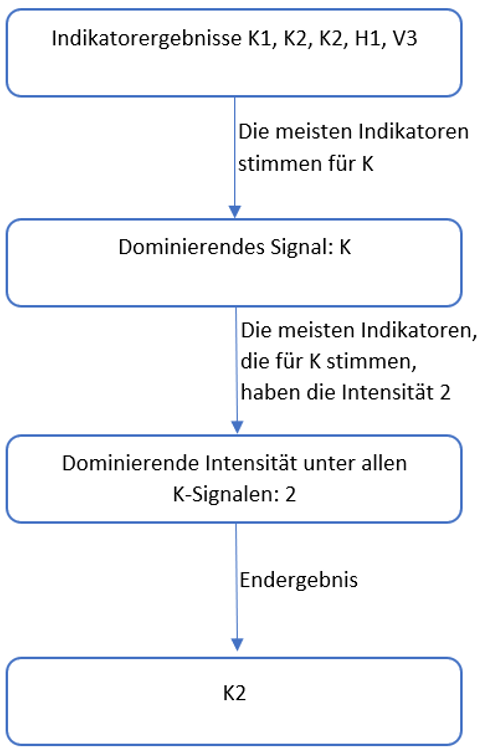
\includegraphics[width=\linewidth]{wahlverfahren}
  \caption{Beispiel für das Wahlverfahren}
  \label{exampleElection}
\end{figure}
\section{Transaktionsempfehlung}

Zu einem gewissen Zeitpunkt ist es unerlässlich, für die Papiere in Abhängigkeit der aus den Indikatoren gewonnenen Signale, konkrete Kaufs- und Verkaufsempfehlungen zu geben. Die hierzu entwickelte Methode liefert also eine Empfehlung zurück, welche Produkte gekauft oder verkauft werden sollen und zu welchem Prozentsatz. Da es in den folgenden Situationen eine Vielzahl von unterschiedlichen Möglichkeiten gibt, macht es Sinn, diese Möglichkeiten in Form eines Zustandsdiagrammes für einen bestimmten Zeitraum darzustellen, um eine gewisse Übersichtlichkeit zu gewährleisten.\cite{ZDiagramm}

Ein Zustandsdiagramm besteht aus einem Startzustand, verschiedenen Zwischenzuständen, Zustandsübergängen, die bei Erfüllung logischer Bedingungen zu Zustandswechseln führen und einem oder mehreren Endzuständen. Startzustände werden durch einen schwarz gefüllten Kreis dargestellt, Endzustände genauso, nur das diese zusätzlich durch einen schwarzen Kreis umrandet sind. Alle anderen Zustände sind durch abgerundete Rechtecke ohne Füllfarbe gekennzeichnet. Die Zustandsübergänge werden durch Pfeile symbolisiert, wobei der Übergang in Pfeilrichtung stattfindet.\cite{ZDiagramm}

Beim Aufruf werden ein Array mit Namen und  ein weiteres mit den entsprechenden Kauf-, Verkauf- und Haltesignalen der Produkte erzeugt. Zurückgegeben wird ein dreidimensionales Array, bestehend aus dem Produktnamen, den Buchstaben K oder V und einer Zahl größer als Null und kleiner gleich Eins zur prozentualen Verarbeitung. Die Buchstaben K und V stehen steht dabei für Kauf und Verkauf.             
\begin{lstlisting}[breakatwhitespace=false, breaklines=true]

	def getTransactions(arrayNames, arrayState,amountToBuy):

\end{lstlisting}
\subsection{Verkauf}
Es macht Sinn, die Höhe der prozentualen Verkaufsempfehlungen an den Bot sowohl von der Stärke des Verkaufs- bzw. Haltesignals des betrachteten Papieres als auch von der Intensität des Kaufsignals anderer Produkte abhängig zu machen. Anhand des stärksten Verkaufssignals wird gemessen, bei welchen Signalwerten gehalten oder verkauft wird und in welchem Ausmaß. Die Folge davon ist, dass dem Bot in der Regel mehr Geld zur Verfügung steht, wenn sich eine besonders gewinnversprechende Möglichkeit auftut. Außerdem werden so wahrscheinlich potentere Papiere in der Regel nicht zugunsten von schlechteren Kaufoptionen verkauft. Die unterschiedlichen Zustände, die durch die Intensität des stärksten Kaufsignals beim Verkauf erzeugt werden können, sind in Abbildung ~\ref{diagrammV} zu sehen. Tabelle ~\ref{tabelleV} zeigt, welche Papiere in den unterschiedlichen Fällen konkret verkauft werden.

\begin{figure}[h]
  \centering
  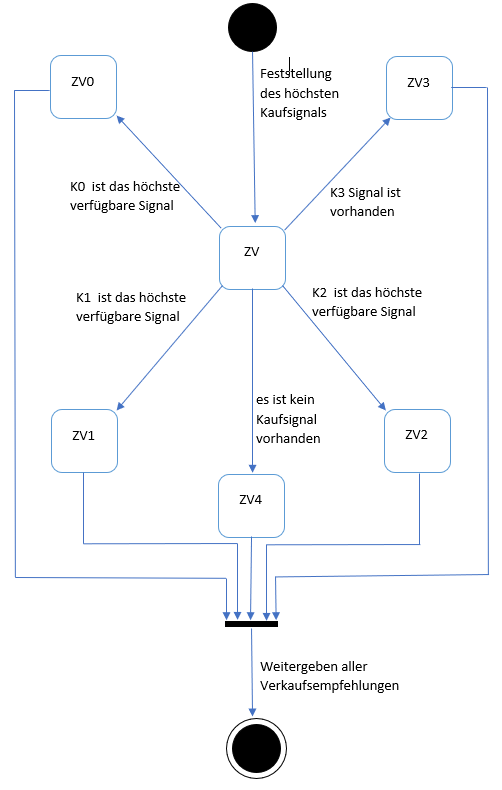
\includegraphics[width=\linewidth]{diagrammVerkauf}
  \caption{Zustandsdiagramm Verkauf}
  \label{diagrammV}
\end{figure}

\begin{figure}[h]
  \centering
  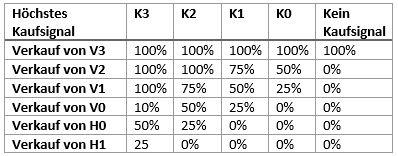
\includegraphics[width=\linewidth]{tabelleVerkauf}
  \caption{Verkauf anhand des höchsten Kaufsignals}
  \label{tabelleV}
\end{figure}

\subsection{Kauf}
Die Auswahl der zu kaufenden Papiere ist logischerweise größtenteils davon abhängig, ob und wie stark das individuelle Kaufsignal ist. Es ist jedoch auch relevant, in wie viele unterschiedliche Produkte der Benutzer investieren möchte. Dennoch werden natürlich die lukrativsten Optionen bevorzugt gekauft, je nach Benutzereingabe aber in unterschiedlichem Ausmaß. Das kann dazu führen, dass nicht hundert Prozent des täglich verfügbaren Kapitals nutzbar ist. Durch die große Variation an Kombinationen von unterschiedlich starken Kaufsignalen entsteht eine große Anzahl an unterschiedlichen Zuständen. Jedoch ist keiner dieser Zustände durch das Setzen der zuvor erwähnten Benutzereingabe statisch, da auch hier mehrere Unterzustände zu verzeichnen sind.

Um das System zu verdeutlichen, wird in Abbildung ~\ref{diagrammK} nur ein Teil des Zustandsdiagramms dargestellt. Angenommen, das höchste Kaufsignal zu einem bestimmten Zeitpunkt ist ein oder mehrere K2, so spielt es für die prozentuale Verteilung auch eine Rolle, ob K1 und oder K0 Papiere vorhanden sind und in welcher Menge, sofern mit K2 nicht der vorgegebene Bedarf gedeckt werden kann.

\begin{figure}[h]
  \centering
  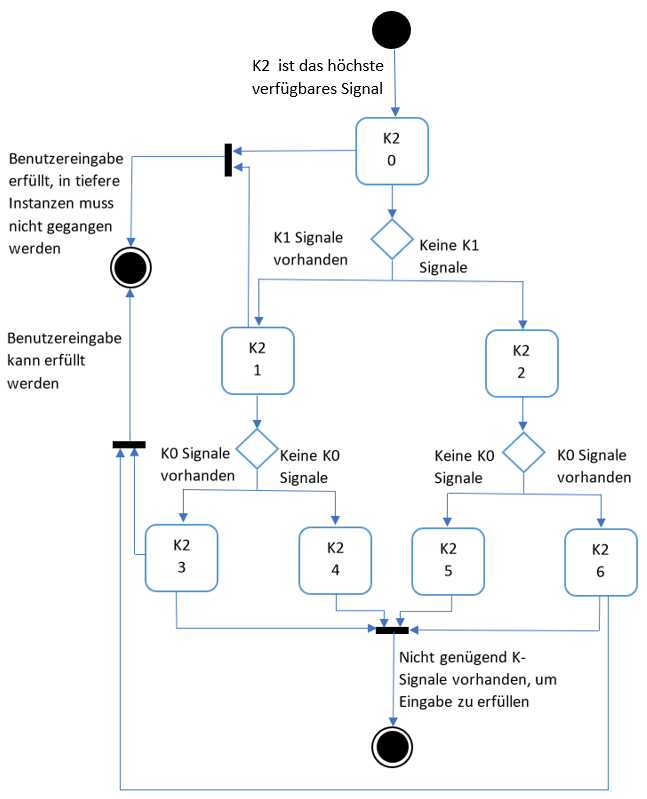
\includegraphics[width=\linewidth]{diagrammKauf}
  \caption{Zustandsdiagramm Kauf}
  \label{diagrammK}
\end{figure}

\end{document}



